\newpage
\chapter{Numerics}

\section{Numerical Spaces}

\subsection{Hilbert Space}
\subsection{Sobolev Space}
\subsection{Banach Space}
\subsection{Krylov Space}

\section{Orthogonalisation}
\subsection{Gram-Schmidt process}

In linear algebra the \textbf{Gram-Schmidt algorithm} is a way of finding two
or more vectors perpendicular to each other. It is a method of constructing an
orhtonormal basis form a set of vectors in  an inner product space, most commonly
the Euclidean space $ \mathbb{R}^n $ equipped with a standard inner product.

The Gram-Schmidt process takes a dinite, \textit{linearly independent} set of
vectors $ \mathbf{S} = \left\{ \mathbf{v}_1, \dots, \mathbf{v}_k \right\} $ for $ k \le n $ and
generates an \textbf{orthogonal} set $ \mathbf{S}' = \left\{ \mathbf{u}_1, \dots, \mathbf{u}_n \right\} $
that spans the same $ k $-dimensional subspace of $ \mathbb{R}^n $ as $ \mathbf{S} $.

The application of the Gram-Schmidt process to the column vectors of a full
column rank matrix yields the \textbf{QR decomposition}.

The vector projection of a vector $ \mathbf{v} $ onto $ \mathbf{u} $ is defined as:

\begin{equation}
    proj_\mathbf{u}(\mathbf{v}) =
    \frac{\left< \mathbf{v}, \mathbf{u} \right>}
    {\left< \mathbf{u}, \mathbf{u} \right>} \mathbf{u}
\end{equation}

where $ \left< \mathbf{v}, \mathbf{u} \right> $ denotes the \textbf{dot product}
of the vectors $ \mathbf{u} $ and $ \mathbf{v} $. This means that the $ proj_\mathbf{u}(\mathbf{v}) $
is the orthogonal projection of $ \mathbf{v} $ onto the line spanned by
$ \mathbf{u} $. It can be also thought of as the part of the vector $ \mathbf{v} $
that is common with vector $ \mathbf{u} $. If the two vectors are perpendicular,
then the dot product is equal 0.

By subtracting the $ proj_\mathbf{u}(\mathbf{v}) $ from vector $ \mathbf{v} $ we
obtain a new vector that is perpendicular to the vector $ \mathbf{u} $.


\begin{figure}[ht]
    \centering
    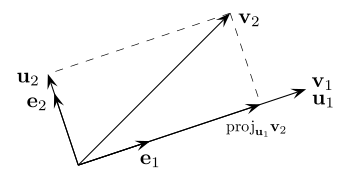
\includegraphics[width=0.8\textwidth]{img/GramSchmidtWiki.png}
    \caption{first two steps of the Gram-Schmidt process}
    \label{fig:Gram-Schmidt-Process-png}
\end{figure}

Given $ k $ nonzero linearly independent vectors $ \mathbf{v}_1, \dots, \mathbf{v}_k $ the
\textbf{Gram-Schmidt} process defines the vectors $ \mathbf{u}_1, \dots, \mathbf{u}_k $
as follows:

\begin{eqarray}
    \mathbf{u}_1 &= \mathbf{v}_1 & \mathbf{e}_1 &= \frac{\mathbf{u}_1}{\norm{\mathbf{u}_1}} \\
    \mathbf{u}_2 &= \mathbf{v}_2 - proj_{\mathbf{u}_1}(\mathbf{v}_2) & \mathbf{e}_2 &= \frac{\mathbf{u}_2}{\norm{\mathbf{u}_2}} \\
    \mathbf{u}_3 &= \mathbf{v}_3 - proj_{\mathbf{u}_1}(\mathbf{v}_3) - proj_{\mathbf{u}_2}(\mathbf{v}_3) & \mathbf{e}_3 &= \frac{\mathbf{u}_3}{\norm{\mathbf{u}_3}} \\
    \quad & \vdots & \quad & \vdots \\
    \mathbf{u}_i &= \mathbf{v}_i - \sum_{j=1}^{i-1} proj_{\mathbf{u}_j}(\mathbf{v}_i) & \mathbf{e}_i &=  \frac{\mathbf{u}_i}{\norm{\mathbf{u}_i}} \\
\end{eqarray}

The sequence $ \mathbf{u}_1, \dots , \mathbf{u}_k $ is the required system of
orthogonal vectors, and the normalised vectors $ \mathbf{e}_1, \dots, \mathbf{e}_k $
form an \textbf{orthonormal set}. The calculation of  $ \mathbf{u}_1, \dots , \mathbf{u}_k $
is known as \textbf{Gram-Schmidt orthogonalisation} and the calculation of sequence
$ \mathbf{e}_1, \dots , \mathbf{e}_k $ is called \textbf{Gram-Schmidt orthonormalisation}.

Python implementation:

\begin{python}
import numpy as np

def GramSchmidtRows(A: np.ndarray, normalise: bool = False):
    """Perform the Gram-Schmidt algorithm on the rows of matrix A so that all
    rows are orthogonalised to the preceding rows"""

    # copy the matrix
    G = A.copy()

    # row to orthogonalise
    for j in range(1, G.shape[0]):
        # the predecessors
        for i in range(j):
            # unit vector representation of preceding row
            unit_row = G[i,:] / np.linalg.norm(G[i,:])
            # projection of current row onto the preceding rows
            G[j,:] -= unit_row * np.dot(G[j,:], unit_row)
        if normalise:
            G[j,:] /= np.linalg.norm(G[j,:])

    return G

def GramSchmidtCols(A: np.ndarray, normalise : bool = False):
    """Perform the Gram-Schmidt algorithm on the columns of matrix A so that all
    columns are orthogonalised to the preceding rows"""

    # copy the matrix
    G = A.copy()

    # column to orthogonalise
    for j in range(1, G.shape[1]):
        # the predecessors
        for i in range(j):
            # unit vector representation of preceding column
            unit_col = G[:,i] / np.linalg.norm(G[:,i])
            # projection of current column onto the preceding columns
            G[:,j] -= unit_col * np.dot(G[:,j], unit_col)
        if normalise:
            G[j,:] /= np.linalg.norm(G[j,:])

    return G
\end{python}


\subsection{Modified Gram-Schmidt process}

The \textbf{Gram-Schmidt orthogonalisation} is prone to \textbf{rounding errors} and
is therefore considered \textbf{numerically unstable}. For the process as described
above it is considered particularly bad.

The \textbf{Gram-Schmidt process} can be stabilised by a small modification, sometimes
referred to as \textbf{modified Gram-Schmidt process} or MGS. This approach
gives the same result as the original formula in exact arithmetic and introdices
smaller errors in finite-precision arithmethic.

Instead of computing the $ \mathbf{u}_i $ as:

\begin{equation}
    \mathbf{u}_i = \mathbf{v}_i - \sum_{j=1}^{i-1} proj_{\mathbf{u}_j}(\mathbf{v}_i)
\end{equation}

it is computed as:

\begin{eqarray}
    \mathbf{u}_{i}^{(1)} &= \mathbf{v}_i - proj_{\mathbf{u}_1}(\mathbf{v}_i) \\
    \mathbf{u}_{i}^{(2)} &= \mathbf{u}_{i}^{(1)} - proj_{\mathbf{u}_2}(\mathbf{u}_{i}^{(1)}) \\
                         & \vdots \\
    \mathbf{u}_{i}^{(i-1)} &= \mathbf{u}_{i}^{(i-2)} - proj_{\mathbf{u}_{i-1}}(\mathbf{u}_{i}^{(i-2)}) \\
    \mathbf{e}_i &= \frac{\mathbf{u}_{i}^{(i-1)}}{\norm{\mathbf{u}_{i}^{(i-1)}}}
\end{eqarray}

Another description would be that the orthogonalisation is performed as a multistep process
where in first step all vectors but first are made orthogonal to the first vectors,
in the second step all vectors but the first two are made orthogonal to the second vector
(already orthogonal to 1st one), and so on untill all are processed.

Python implementation:

\begin{python}
import numpy as np

def ModifiedGramSchmidtRows(A: np.ndarray, normalise: bool = False):
    """Perform the Modified Gram-Schmidt algorithm on the rows of matrix A
    so that all rows are orthogonalised to the preceding rows"""

    # copy the matrix
    G = A.copy()

    # vector to orthogonalise against
    for i in range(G.shape[0]-1):
        # simplify dot product
        unit_row = G[i,:] / np.linalg.norm(G[i,:])
        if normalise:
            G[i,:] = unit_row
        # all later vectors
        for j in range(i+1, G.shape[0]):
            # subtract the projection
            G[j,:] -= unit_row * np.dot(G[j,:], unit_row)

    return G

def ModifiedGramSchmidtCols(A: np.ndarray, normalise: bool = False):
    """Perform the Modified Gram-Schmidt algorithm on the columns of matrix A
    so that all columns are orthogonalised to the preceding rows"""

    # copy the matrix
    G = A.copy()

    # vector to orthogonalise against
    for i in range(G.shape[1]-1):
        # simplify dot product
        unit_col = G[:,i] / np.linalg.norm(G[:,i])
        if normalise:
            G[:,i] = unit_col
        # all later vectors
        for j in range(i+1, G.shape[1]):
            # subtract the projection
            G[:,j] -= unit_col * np.dot(G[:,j], unit_col)

    return G
\end{python}


\section{Factorisation}

\subsection{Cholesky Factorisation}

Cholesky Factorisation is a matrix operation such that a matrix $ \m{A} $ is
decomposed to a multiplication of a lower triangular martrix $ \m{L} $ and its
conjugate transpose $ \m{L}^T $.

The \textbf{Cholesky Factorisation} is applicable to a \textbf{Hermitian},
\textbf{positive definite} matrices.

\begin{equation}
    \m{A} = \m{L} \m{L}^*
\end{equation}

Every Hermitian positive definite matrix (and thus every real-valued symmetric
positive definite matrix) has a unique Cholesky factorisation.

If $ \m{A} $ can be written as $ \m{L} \m{L}^* $ for some invertible $ \m{L} $,
lower triangular or otherwise, then $ \m{A} $ is Hermitian and positive definite.

When $ \m{A} $ is a real matrix (hence symmetric and positive definite), the
factorisation may be written:

\begin{equation}
    \m{A} = \m{L} \m{L}^T
\end{equation}

A Python example of \textit{Cholesky-Banachiewicz} factorisation algorithm:

\begin{python}
import numpy as np

def Cholesky_Banachiewicz(A: np.ndarray) -> np.ndarray:
    """Perform the Choleski factorisation of matrix A such that:

    A = L @ L.T

    where:
        L is lower triangular matrix

    Args:
        A (np.ndarray): a real, symmetric, positive-definite matrix

    Returns:
        (np.ndarray): the result of the decomposition stored as a lower triangular
        matrix.
    """
    L = np.zeros(A.shape, dtype=A.dtype)
    for i in range(A.shape[0]):
        for j in range(i+1):
            sum = 0
            for k in range(j):
                sum += L[i,k] * L[j,k]

            if i == j:
                L[i,j] = np.sqrt(A[i,i] - sum)
            else:
                L[i,j] = 1. / L[j,j] * (A[i,j] - sum)

    return L
\end{python}

And the solution of matrix equation:

\begin{eqarray}
    \mathbf{A} \mathbf{x} &= \mathbf{b} \\
    \mathbf{A} &= \mathbf{L} \mathbf{L}^T \\
    \mathbf{L} \mathbf{L}^T \mathbf{x} &= \mathbf{b} \quad , substitute \quad \mathbf{y} = \mathbf{L}^T \mathbf{x} \\
    \mathbf{L} \mathbf{y} &= \mathbf{b} \quad,\ solve\ using\ forward\ substitution \\
    \mathbf{L}^T \mathbf{x} &= \mathbf{y} \quad,\ solve\ using\ backward\ substitution
\end{eqarray}

the $ \mathbf{b} $ can be either a vector or a matrix.

Python example:

\begin{python}
import numpy as np

def Solve_Triangular(A: np.ndarray, b: np.ndarray, kind="lower") -> np.ndarray:
    """Solve Ax = b using either forward or backward substitution. For lower
    triangular matrix the forward substitution is used, for upper triangular
    matrix the backward substitution is used.
    """
    b = b.copy()
    flatten = False
    if len(b.shape) == 1:
        b = b.reshape(-1,1)
        flatten = True

    m = A.shape[0]
    n = b.shape[1]
    x = np.zeros(b.shape, dtype=b.dtype)

    if kind == "lower":
        for i in range(m):                # rows of A
            x[i,:] = b[i,:]               # perform operations on whole row of b
            for j in range(i):            # columns of A from start to diagonal
                x[i,:] -= A[i,j] * x[j,:] # perform operations on whole row of b
            x[i,:] /= A[i,i]              # divide by the element on the diagonal

    elif kind == "upper":
        for i in reversed(range(m)):      # rows of A from end
            x[i,:] = b[i,:]               # perform operations on whole row of b
            for j in range(i+1, m):       # columns of A from diagonal up to end
                x[i,:] -= A[i,j] * x[j,:] # perform operations on whole row of b
            x[i,:] /= A[i,i]              # divide by the element on the diagonal

    else:
        raise NotImplementedError(f"Substitution for other than 'lower' or 'upper' triangular not implemented: '{kind:s}'.")

    if flatten:
        return x.flatten()
    else:
        return x


def Cholesky_Solve(L: np.ndarray, b: np.ndarray) -> np.ndarray:
    """Solve the matrix equation using results of Cholesky decomposition

        Ax = b
        A = L @ L.T
        L @ L.T @ x = b
        L @ z = b
        L.T @ x = z

    Args:
        L (np.ndarray): a lower triangular matrix from Cholesky decomposition
        b (np.ndarray): right hand side of the equation

    Returns:
        (np.ndarray): the solution on the left hand side
    """
    z = Solve_Triangular(L,   b, "lower")
    x = Solve_Triangular(L.T, z, "upper")
    return x

\end{python}


\subsection{LU Factorisation}

\subsubsection{LU Factorsation without pivoting}
\subsubsection{LU Factorsation with row pivoting}
\subsubsection{LU Factorsation with complete pivoting}

\subsection{QR Factorisation}

\subsubsection{QR Factorisation using Gram-Schmidt algorithm}
\subsubsection{QR Factorisation using Givens rotations}
\subsubsection{QR Factorisation using Householder reflections}
\subsubsection{QR Factorisation using Householder reflections with column pivoting}

\subsection{Converson to Hessenberg tridiagonal form using Givens rotations}
\subsection{Converson to Hessenberg tridiagonal form using Householder reflections}
\subsection{Converson to Hessenberg tridiagonal form using Jacobi rotations}

\subsection{Jacobi rotations to diagonal matrix}
\subsection{Arnoldi algorithm}
\subsection{Lanczos algorithm}
\subsection{Schur algorithm}

\subsection{Singular Value Decomposition (SVD)}
\subsubsection{SVD using Power Iteration}
\subsubsection{SVD using QR (orthogonal) Iteration}


\subsection{Positive semidefinite matrices}

If a Hermitian matrix $ \m{A} $ is only positive semidefinite, instead of positive
definite, then it still has a decomposition of the form $ \m{A} = \m{L} \m{L}^* $
where the diagonal entries of $ \m{L} $ are allowed to be zero. The decompostion
need not be unique, for example:

\begin{equation}
    \begin{bmatrix}
        0 & 0 \\
        0 & 1\\
    \end{bmatrix}
    = \m{L} \m{L}^*
\end{equation}

\begin{equation}
    \m{L} =
    \begin{bmatrix}
        0 & 0 \\
        \cos \theta & \sin \theta
    \end{bmatrix}
\end{equation}

However, if the rank of $ \m{A} $ is $ r $, then there is a unique lower triangular
$ \m{L} $ with exactly $ r $ positive diagonal elements adn $ n - r $ columns
containing all zeros.

Alternatively, the decomposition can be made unique when  a pivoting choice is
fixed. Formally, if $ \m{A} $ is an $ n \times n $ positive semidefinite matrix
of rank $ r $, then there is at least one permutation matrix $ \m{P} $ such
that $ \m{P} \m{A} \m{P}^T $ has a unique decompostion of the form

\begin{equation}
    \m{P} \m{A} \m{P}^T = \m{L} \m{L}^*
\end{equation}

with

\begin{equation}
    \m{L} = \begin{bmatrix}
        \m{L}_1 & \m{0} \\
        \m{L}_2 & \m{0} \\
    \end{bmatrix}
\end{equation}

where $ \m{L}_1 $ is a $ r \times r $ lower triangular matrix with positive
diagonal.


\subsubsection{Example}

\begin{equation}
    \begin{bmatrix}
        \phantom{-1}4 & \phantom{-}12 & -16 \\
        \phantom{-}12 & \phantom{-}37 & -43 \\
        -16 & -43 & \phantom{-}98 \\
    \end{bmatrix}
    = \begin{bmatrix}
        \phantom{-}2 & 0 & 0 \\
        \phantom{-}6 & 1 & 0 \\
        -8 & 5 & 3 \\
    \end{bmatrix}
    \begin{bmatrix}
        2 & 6 & -8 \\
        0 & 1 & \phantom{-}5 \\
        0 & 0 & \phantom{-}3 \\
    \end{bmatrix}
\end{equation}


\subsection{Applications}

\textbf{Solution of a system of linear equations}

The Cholesky decomposition is mainly used for the numerical solution of
\textbf{linear equations} $ \m{A} \m{x} = \m{b} $. If $ \m{A} $ is symmetric
and positive definite, then we can solve $ \m{A} \m{x} = \m{b} $ by first computing
the Cholesky decomposition $ \m{A} = \m{L} \m{L}^* $, then solving
$ \m{L} \m{y} = \m{b} $ for $ \m{y} $ by forward substitution and finally solving
$ \m{L}^* \m{x} = \m{y} $ for $ \m{x} $ by back substitution.

\begin{eqarray}
    \m{A} \m{x} &= \m{b} \\
    \m{L} \m{L}^* \m{x} &= \m{b},\ substitute\ \m{L}^* \m{x} = \m{y} \\
    \m{L} \m{y} &= \m{b},\ then\ solve \\
    \m{L}^* \m{x} &= \m{y}
\end{eqarray}

For linear systems that can be put into symmetric form, the Cholesky decomposition
is the method choice, for superior efficiency and numerical stability. Compared
to the \textbf{LU} decomposition, it is roughly twice as efficient.


\subsection{Matrix Inversion}

A non-Hermitian matrix $ \m{B} $ can be inverted using the following identity,
where $ \m{B} \m{B}^* $ will always be Hermitian:

\begin{equation}
    \m{B}^{-1} = \m{B}^* ( \m{B} \m{B}^* )^{-1}
\end{equation}

The above stated matrix relation is also called the \textbf{pseudoinverse}
of a matrix. The following equality holds:

\begin{equation}
    \m{B}^* ( \m{B} \m{B}^* )^{-1} = ( \m{B}^* \m{B} )^{-1} \m{B}^*
\end{equation}

The best way to compute the \textbf{pseudoinverse} is to use
\textbf{singular value decomposition} (\textbf{SVD}). With $ \m{A} $ being
$ \m{A} = \m{U} \m{S} \m{V}^* $,
where $ \m{U} $ and $ \m{V} $ (both $ n \times n $) are
orthogonal and
$ \m{S} $ ( $ m  \times n $ ) is \textbf{diagonal} with real, non-negative
\textit{singular values} $ \sigma_{i,1} = 1, \dots, n $. We find that

\begin{equation}
    \m{A}^* = \m{V} ( \m{S}^* \m{S} )^{-1} \m{S}^* \m{U}^*
\end{equation}

If the rank $ r $ of $ \m{A} $ is smaller than $ n $, the inverse of
$ \m{S}^* \m{S} $ does not exist, and one uses only the first $ r $ singular
values. $ \m{S} $ then becomes an $ r \times r $ matrix and $ \m{U}$, $ \m{V} $
shrink accordingly.


\section{Linear Regression}
\subsection{Derivation}

\textbf{Linear Regression} is an approach for predicting a response using
a \textbf{single feature}. In linear regression we assume that two variables
i. e. independent and dependent are linearly related.

Generalrly we define $ \m{x} $ as a \textbf{feature vector}:

\begin{equation}
    \m{x} = \left[ x_1, x_2, ..., x_n \right]
\end{equation}

and $ \m{y} $ as \textbf{response vector}:

\begin{equation}
    \m{y} = \left[ y_1, y_2, ..., y_n \right]
\end{equation}

then a predicted response:

\begin{equation}
    h(x_i) = \beta_0 + \beta_1 \times x_i
\end{equation}

where: \\
$ x_i $ represents the \textit{i}-th observation \\
$ \beta_1 $ represents the slope, and \\
$ \beta_0 $ represents the intercept of the regression line.


To predict a new value $ y_i $, we need to consider:

\begin{equation}
    y_i = \beta_0 + \beta_1 \times x_i + \epsilon_i = h(x_i) + \epsilon_i
\end{equation}

where:\\
$ \epsilon_i $ is the \textbf{error} of the estimate.

The error function is therefore obtained:

\begin{equation}
    \epsilon_i = y_i - h(x_i)
\end{equation}

The $ \beta_0 $ and $ \beta_1 $ coefficients are obtained by minimizing the residual
\textbf{error} of the estimate using e.g. the \textbf{least square method}:

\begin{eqarray}
    J(\beta_0, \beta_1) &= \frac{1} {2 n} \sum_{i=1}^{n} \epsilon_i^2 \\
    &= \frac{1} {2 n} \sum_{i=1}^{n} \left( y_i - h(x_i) \right)^2 \\
    &= \frac{1} {2 n} \sum_{i=1}^{n} \left( y_i - \beta_0 - \beta_1 \times x_i  \right)^2
\end{eqarray}

To find the coefficients we can derviate the cost function, first with regards to $ \beta_0 $:

\begin{equation}
    \frac{\partial J} {\partial \beta_0} \left[ \frac{1} {2 n} \sum_{i=1}^{n} \left( y_i - \beta_0 - \beta_1 \times x_i  \right)^2 \right] = 0
\end{equation}

where using the chain rule we can write:

\begin{eqarray}
    u &= y_i - \beta_0 - \beta_1 \times x_i \\
    J &= \frac{1} {2 n} \sum_{i=1}^n u^2 \\
    \frac{\partial J} {\partial \beta_0} &= \frac{\partial J} {\partial u} \times \frac{\partial u} {\partial \beta_0} \\
    \frac{\partial J} {\partial u} &= 2 u \\
    \frac{\partial u} {\partial \beta_0} &= -1 \\
    \frac{\partial J} {\partial \beta_0} &= \frac{1} {2n} \times (-2)  \times \sum_{i=1}^n \left(y_i - \beta_0 - \beta_1 \times x_i \right) \\
    0 &= \frac{1} {n} \sum_{i=1}^n \left( y_i - \beta_0 - \beta_1 \times x_i \right) \\
    0 &= \frac{1} {n} \sum_{i=1}^n y_i - \frac{1} {n} \sum_{i=1}^n \beta_0 - \frac{1} {n} \beta_1 \sum_{i=1}^n x_i \\
    0 &= \bar{y}_i - \beta_0 - \beta_1 \bar{x}_i \\
    \beta_0 &= \bar{y} - \beta_1 \bar{x}
\end{eqarray}

To find $ \beta_1 $:

\begin{equation}
    \frac{\partial J} {\partial \beta_1} \left[ \frac{1} {2 n} \sum_{i=1}^{n} \left( y_i - \beta_0 - \beta_1 \times x_i  \right)^2 \right] = 0
\end{equation}

\begin{eqarray}
    u &= y_i - \beta_0 - \beta_1 \times x_i \\
    J &= \frac{1} {2 n} \sum_{i=1}^n u^2 \\
    \frac{\partial J} {\partial \beta_1} &= \frac{\partial J} {\partial u} \times \frac{\partial u} {\partial \beta_1} \\
    \frac{\partial J} {\partial u} &= 2 u \\
    \frac{\partial u} {\partial \beta_1} &= -x \\
    \frac{\partial J} {\partial \beta_1} &= \frac{1} {2 n} \times (-2) \sum_{i=1}^n x_i \times \left( y_i - \beta_0 - \beta_1 x_i \right) \\
    0 &= \frac{1}{n} \sum_{i=1}^n x_i \left( y_i - \beta_0 - \beta_1 x_i \right) \\
    0 &= \frac{1}{n} \sum_{i=1}^n \left( x_i y_i - \beta_0 x_i - \beta_1 x_i^2 \right)
\end{eqarray}

Substituting the value of $ \beta_0 $:

\begin{eqarray}
    \beta_0 &= \bar{y} - \beta_1 \bar{x} \\
    0 &= \frac{1} {n} \sum_{i=1}^n \left(x_i y_i - \left(\bar{y} - \beta_1 \bar{x} \right) x_i - \beta_1 x_i^2 \right) \\
    0 &= \frac{1} {n} \sum_{i=1}^n \left(x_i y_i - \bar{y} x_i + \beta_1 \bar{x} x_i - \beta_1 x_i^2 \right) \\
    0 &= \frac{1} {n} \left( \sum_{i=1}^n \left(x_i y_i - \bar{y} x_i \right) - \beta_1 \sum_{i=1}^n \left(x_i^2 - \bar{x} x_i \right) \right) \\
    \beta_1 &= \frac{\frac{1}{n} \sum_{i=1}^n \left(x_i y_i - \bar{y} x_i \right)}
                    {\frac{1}{n} \sum_{i=1}^n \left(x_i^2 - \bar{x} x_i \right)}
\end{eqarray}

Simplifying the formula using:

\begin{eqarray}
    \bar{y} &= \frac{1}{n} \sum_{i=1}^n y_i \\
    \bar{x} &= \frac{1}{n} \sum_{i=1}^n x_i
\end{eqarray}

we get:
\begin{eqarray}
    \beta_1 &= \frac{\frac{1}{n} \sum_{i=1}^n x_i y_i - \bar{x} \bar{y}}
                    {\frac{1}{n} \sum_{i=1}^n x_i^2 - \bar{x} \bar{x}} \\
    \beta_1 &= \frac{\sum_{i=1}^n x_i y_i - n \bar{x} \bar{y}}
                    {\sum_{i=1}^n x_i^2 - n \bar{x}^2}
\end{eqarray}


\subsection{Result}

\begin{bbox}
    So, to recapitulate, to get a linear regression coefficients for a dataset:

    \begin{eqarray}
        \m{x} &= \left[ x_1, x_2, ..., x_n \right] \\
        \m{y} &= \left[ y_1, y_2, ..., y_n \right]
    \end{eqarray}

    we may use equations:

    \begin{eqarray}
        \beta_1 &= \frac{\sum_{i=1}^n x_i y_i - n \bar{x} \bar{y}}
                        {\sum_{i=1}^n x_i^2 - n \bar{x}^2} \\
        \beta_0 &= \bar{y} - \beta_1 \bar{x}
    \end{eqarray}

    with an error:
    \begin{equation}
        \epsilon_i = y_i - \beta_0 - \beta_1 x_i
    \end{equation}

\end{bbox}


\section{Interpolation and Mapping of Values}

\section{Modal Assurance Criterion (MAC)}

\section{Campbell Diagram, Order Analysis}

\section{Power Spectral Density, Cross Spectral Density and Coherence}

\section{Sorting}

\section{Reverse Cuthill-McKee Algorithm for rearranging Sparse matrix}

\section{Topology Optimization}

\section{Generalised Eigenvalue Problem}




